\begin{frame}
    \titlepage
\end{frame}

\begin{frame}{Índice}
    \tableofcontents
\end{frame}


\section{Introducción}

    \begin{frame}
        \Huge{\centerline{Introducción}}
    \end{frame}

    \begin{frame}{Motivación}
        \begin{itemize}
            \item Plan de inversión de la Agencia Digital de Andalucía para 2022
            \\~\\
            \item Proyecto para estudiantes, desarrollado por un estudiante
            \\~\\
            \item Algo distinto a los CTFs, sin \textit{banderas}
        \end{itemize}
    \end{frame}

    \begin{frame}{Metodología}
        \begin{columns}[c]
            \column{.45\textwidth}
                \begin{itemize}
                    \item Desarrollo incremental
                    \\~\\
                    \item \textit{Getting Things Done}
                    \\~\\
                    \item Gantt y Kanban
                \end{itemize}
            
            \column{.5\textwidth}
                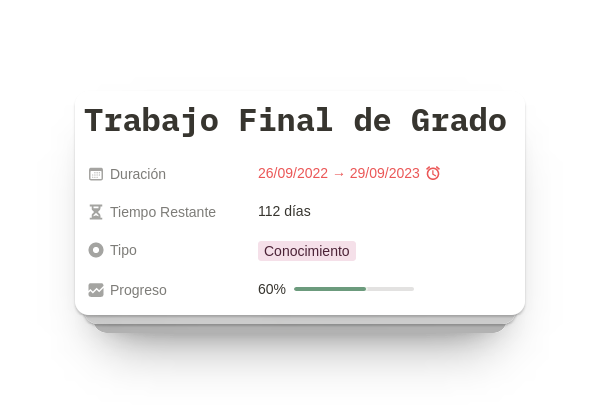
\includegraphics[scale=0.25]{images/capturas/notion/resumen.png}
        \end{columns}
    \end{frame}

    % \begin{frame}
    %     \centering

    %     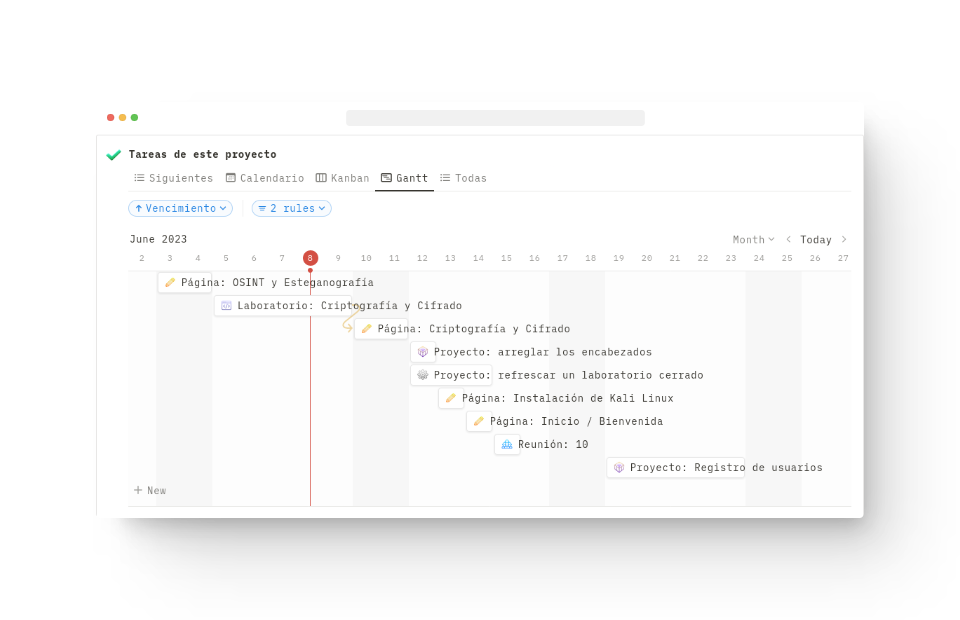
\includegraphics[scale=0.3]{images/capturas/notion/gantt.png}
    % \end{frame}

    % \begin{frame}
    %     \centering

    %     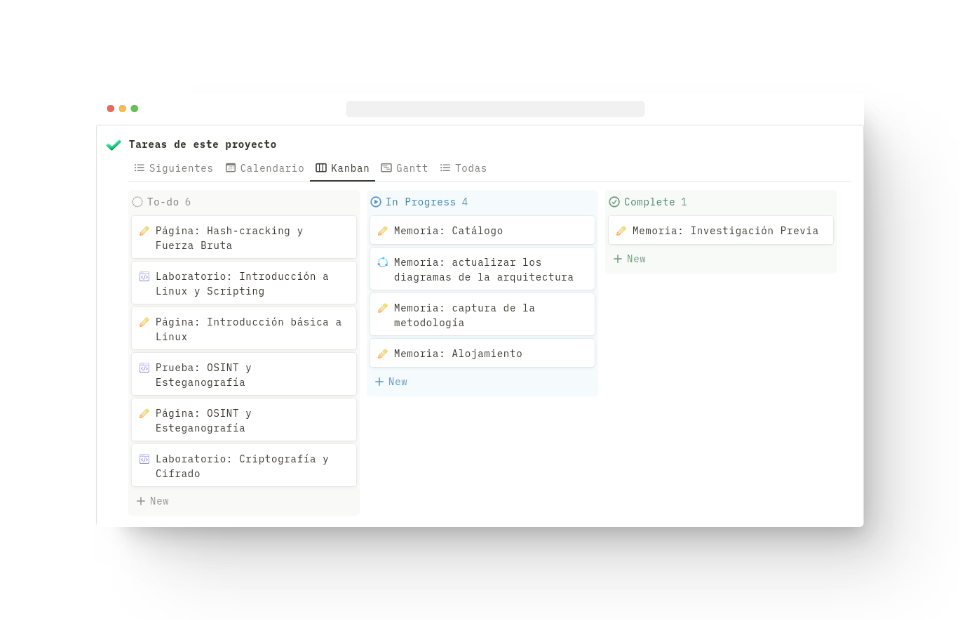
\includegraphics[scale=0.3]{images/capturas/notion/kanban.png}
    % \end{frame}

    \begin{frame}{Estructura global del proyecto}
        \centering

        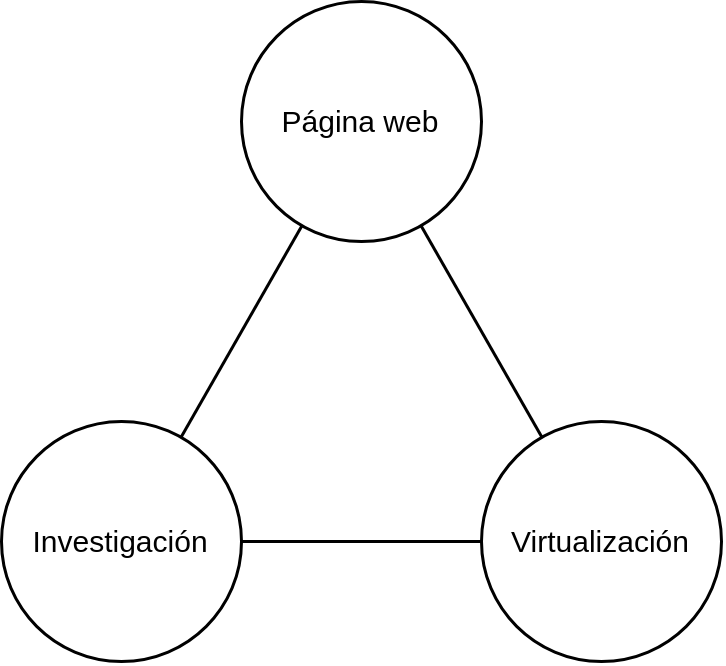
\includegraphics[scale=0.2]{images/diagramas/estructura-global.png}
    \end{frame}


% \section{Investigación previa}

%     \begin{frame}
%         \Huge{\centerline{Investigación previa}}
%     \end{frame}

    \begin{frame}{Proceso creativo}
        \begin{columns}[c]
            \column{.45\textwidth}
                \begin{itemize}
                    \item Plataforma de CTFs
                    \\~\\
                    \item Portal de descargas
                    \\~\\
                    \item \textbf{Laboratorios}
                \end{itemize}
            
            \column{.5\textwidth}
                
\includegraphics[scale=0.25]{images/interrogacion.png}
        \end{columns}
    \end{frame}

    \begin{frame}{Análisis de tecnologías}
        % \centering

        % \includegraphics[scale=0.3]{images/capturas/tabla.png}

        \begin{itemize}
            \item \textbf{Sitio web}: Astro / Wordpress / Drupal
            \\~\\
            \item \textbf{Base de datos}: SQLite / MySQL
            \\~\\
            \item \textbf{Almacenamiento}: Local / Remoto (AWS, Linode, GCP) 
        \end{itemize}
    \end{frame}


\section{Diseño y desarrollo}

    \begin{frame}
        \Huge{\centerline{Diseño y desarrollo}}
    \end{frame}

    \begin{frame}{Arquitectura}
        \centering

        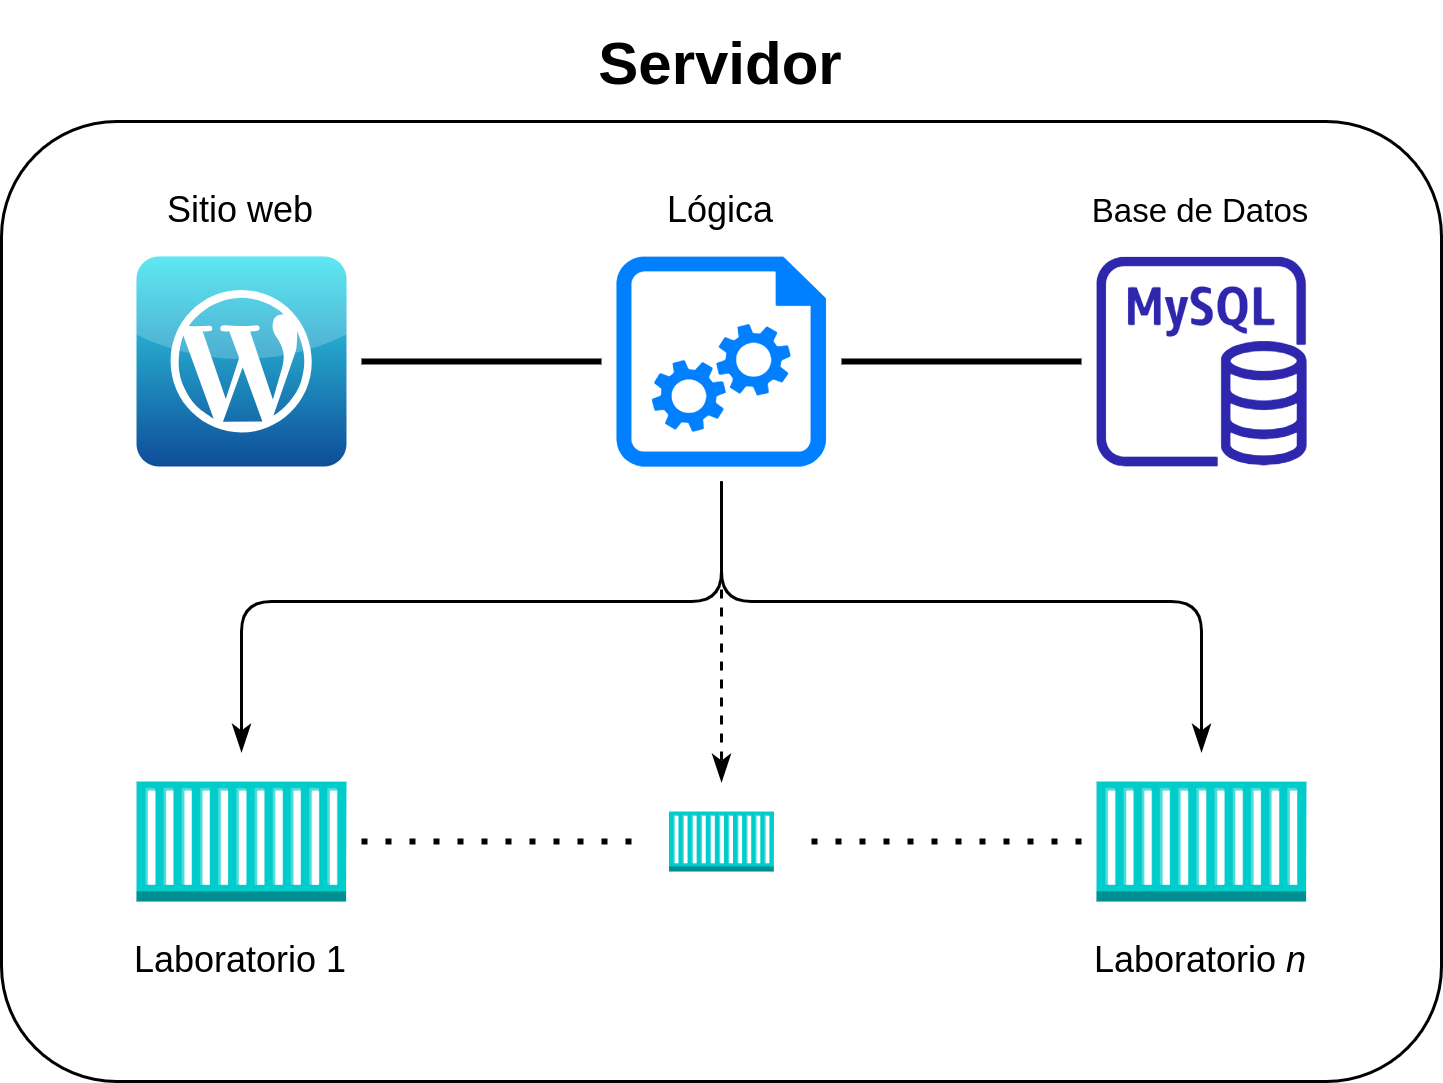
\includegraphics[scale=0.15]{images/diagramas/arquitectura.png}
    \end{frame}

    \begin{frame}{Modelado de procesos}
        \centering

        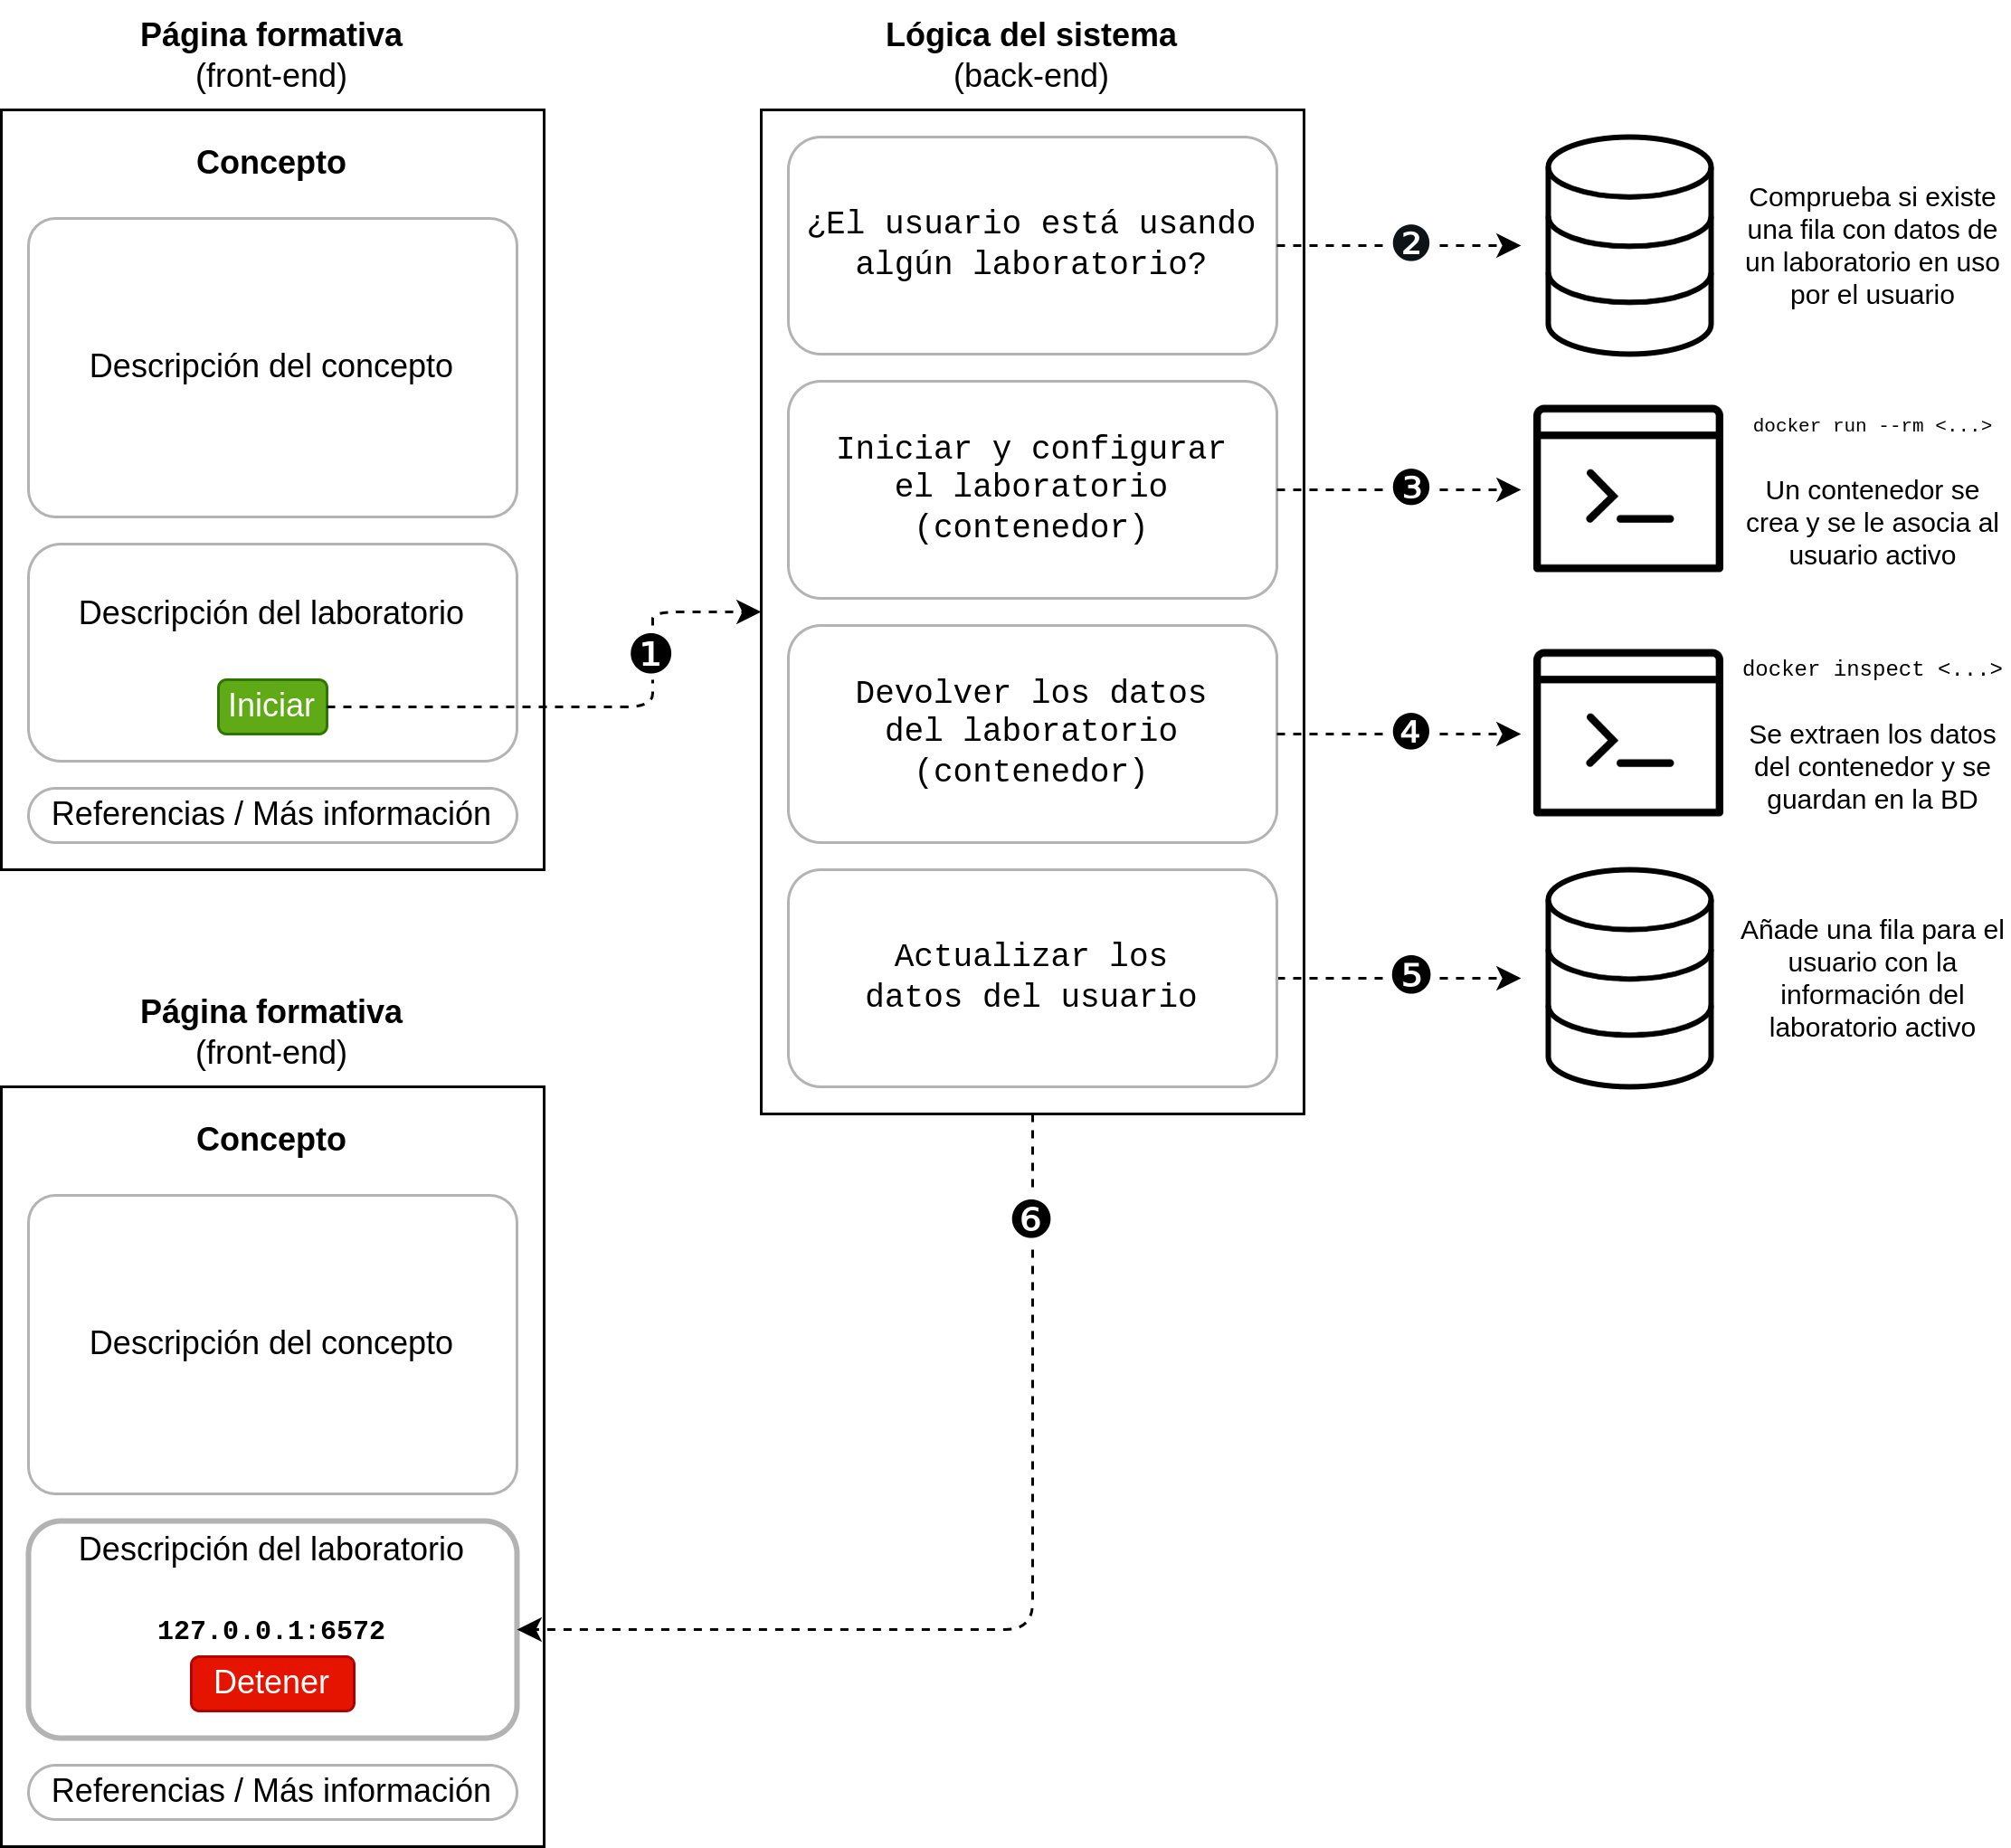
\includegraphics[scale=0.09]{images/diagramas/iniciar.png}
    \end{frame}

    \begin{frame}
        \centering

        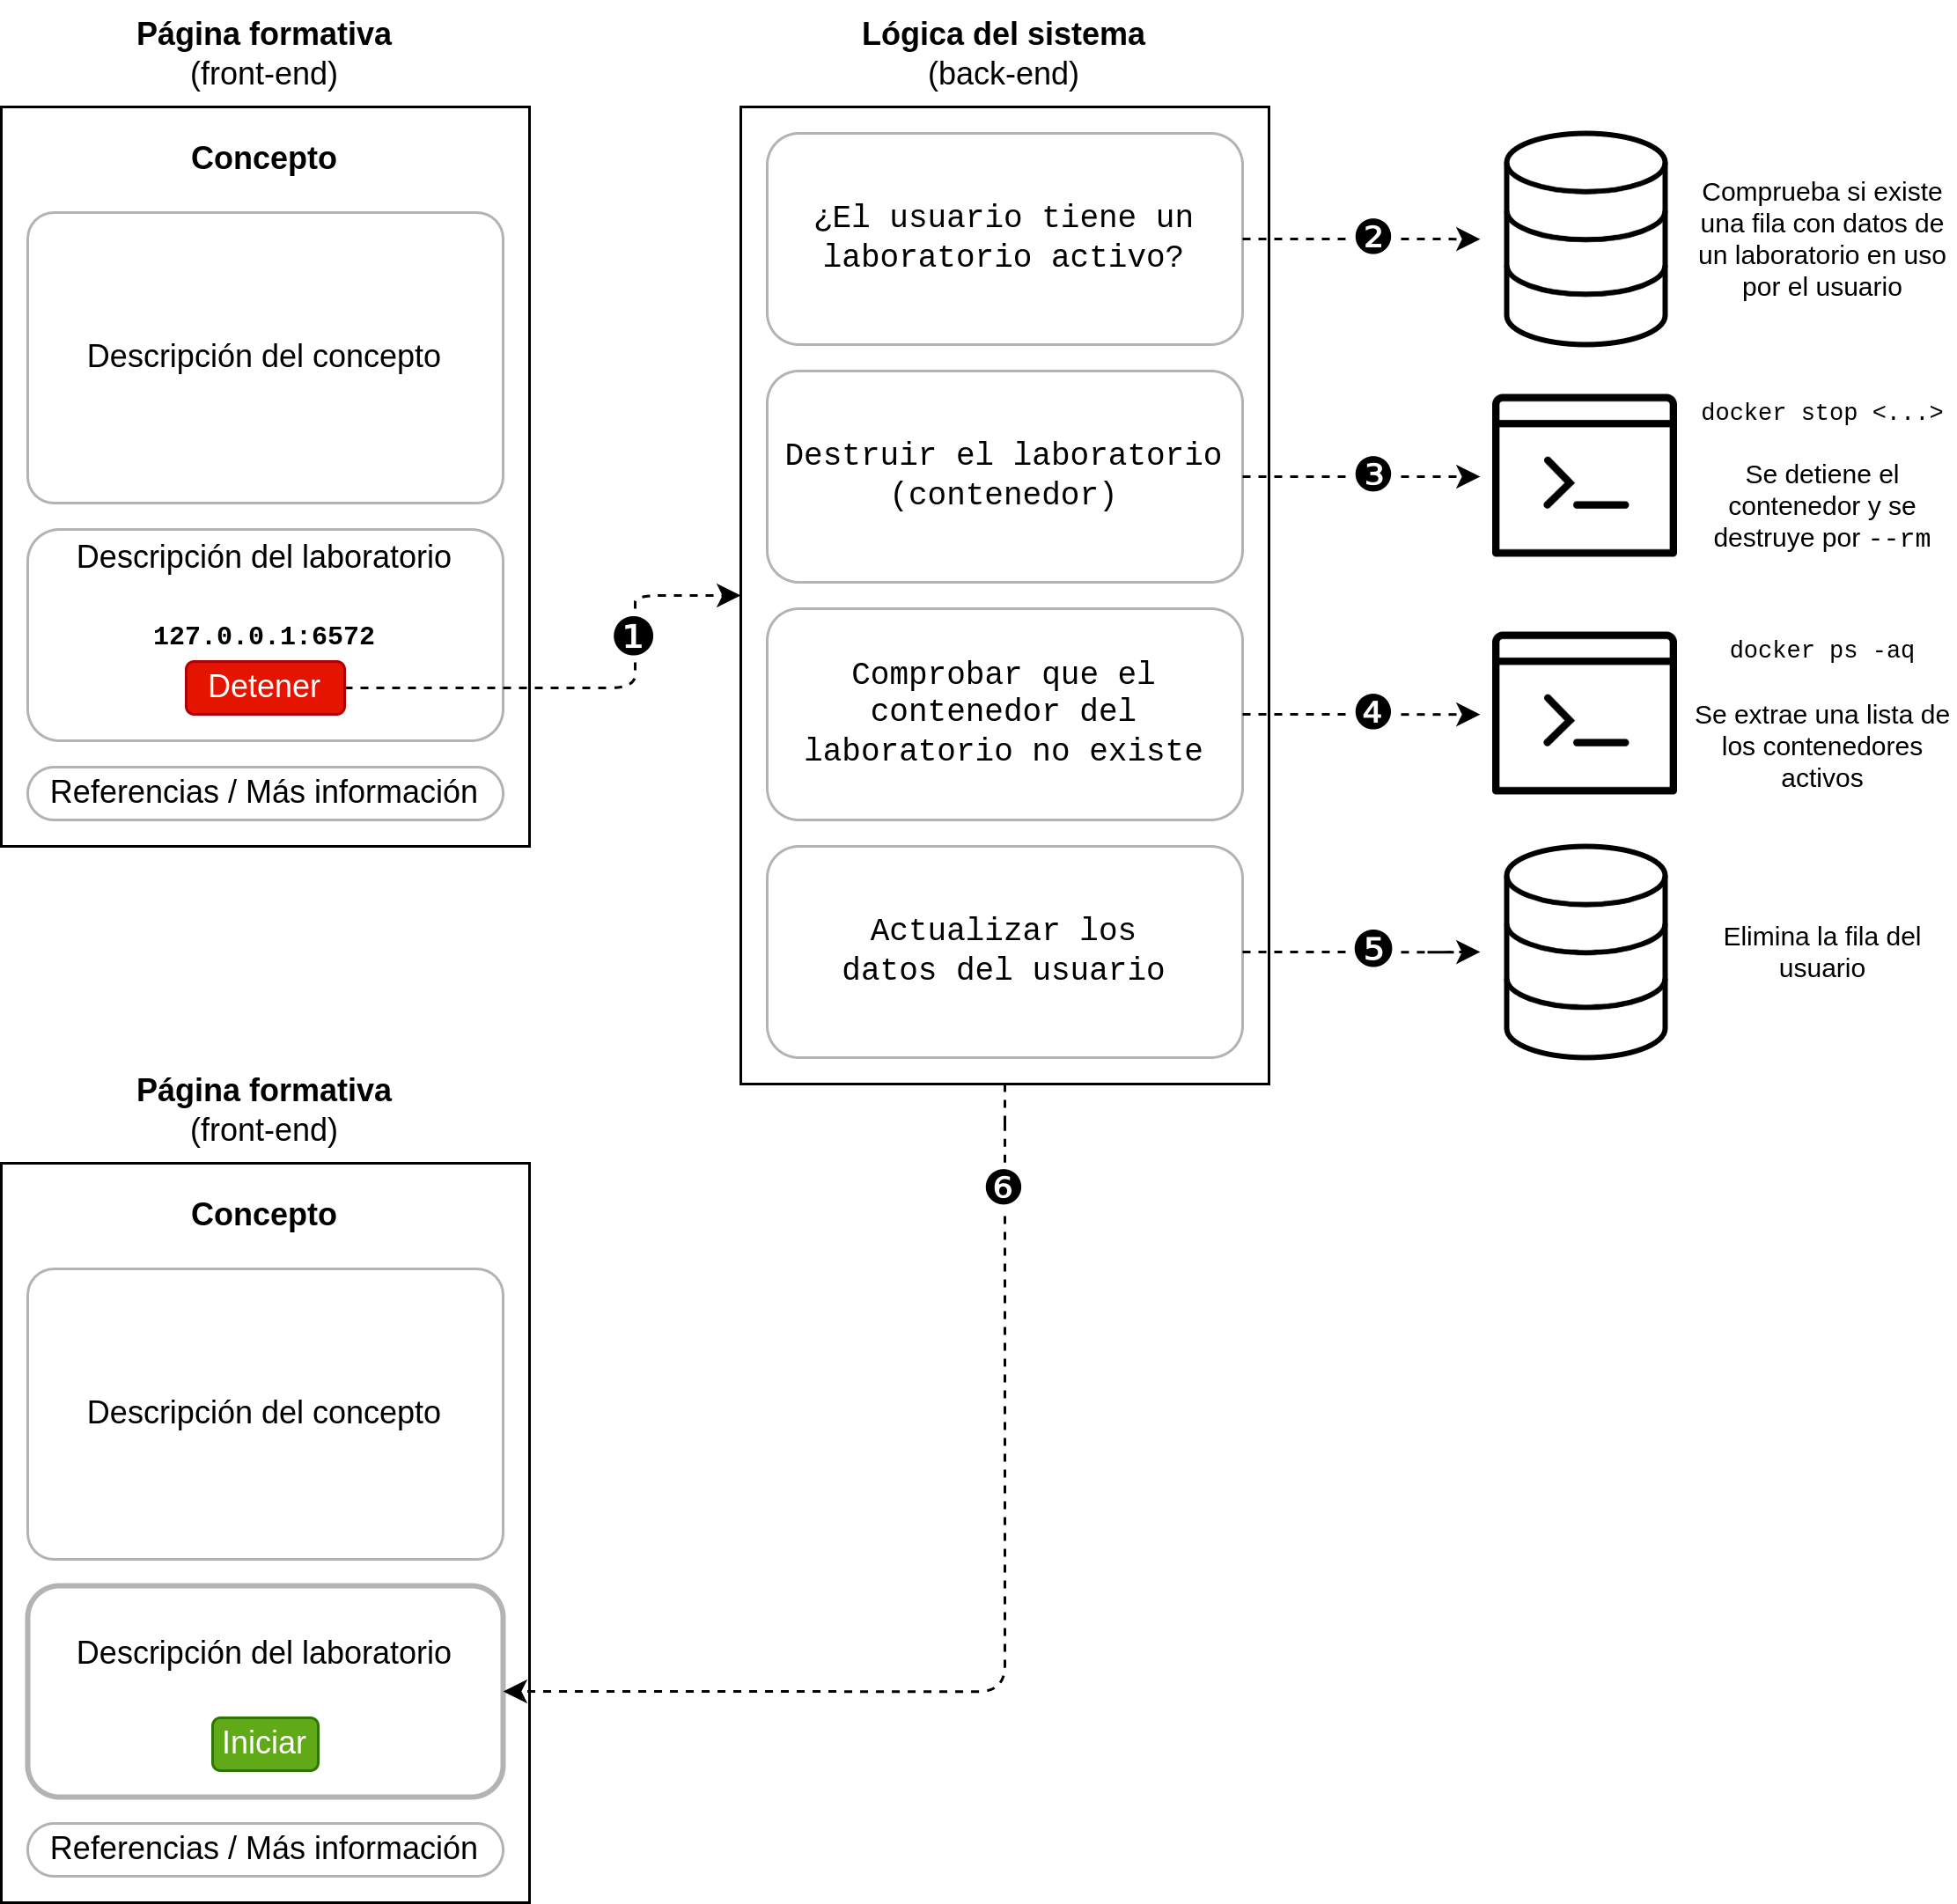
\includegraphics[scale=0.09]{images/diagramas/detener.png}
    \end{frame}

    \begin{frame}
        \centering

        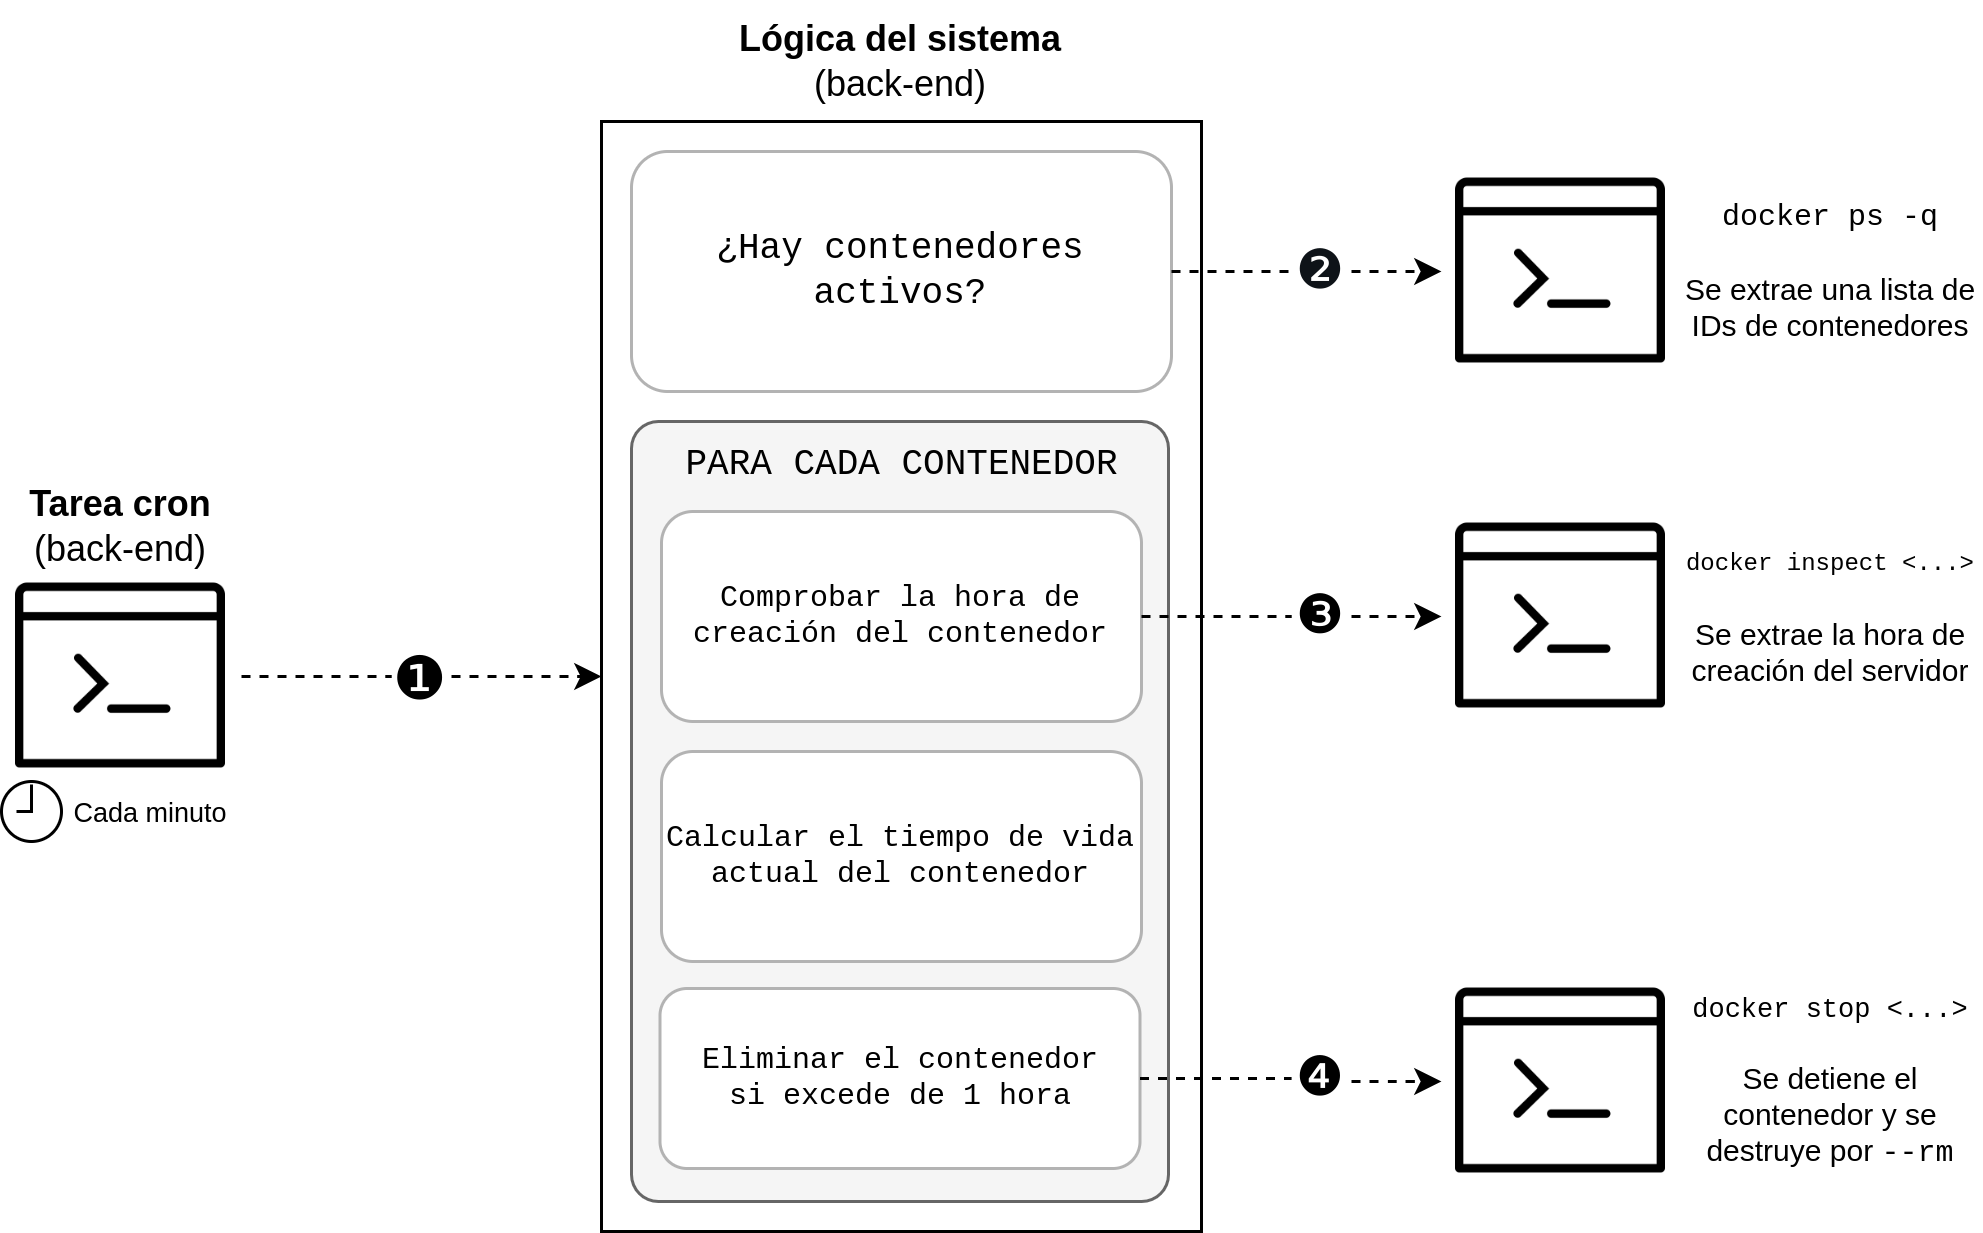
\includegraphics[scale=0.15]{images/diagramas/cron.png}
    \end{frame}


\section{Catálogo de conceptos}

    \begin{frame}
        \Huge{\centerline{Catálogo de conceptos}}
    \end{frame}

    \begin{frame}{Laboratorios de introducción}
        \begin{block}{Linux}
            Jerarquía de ficheros y directorios, y gestión de usuarios y permisos.
        \end{block}
        \begin{block}{Bash}
            Sintaxis básica, variables, condicionantes, bucles y funciones.
        \end{block}

        \begin{block}{Redes}
            Protocolos, tipos y topologías de red, y ataques más comunes.
        \end{block}

        \begin{block}{OSINT}
            Descripción y herramientas útiles de recolección de información.
        \end{block}
    \end{frame}
    
    \begin{frame}{Laboratorios normales}
        \begin{block}{Análisis de tráfico}
            Captura de tráfico, paquetes y herramientas.
        \end{block}

        \begin{block}{Esteganografía}
            Definición y herramientas comunes.
        \end{block}

        \begin{block}{Fuerza bruta}
            Definición y puesta en práctica.
        \end{block}

        \begin{block}{Hash-cracking}
            Descripción y herramientas comunes.
        \end{block}
    \end{frame}
    
    \begin{frame}
        \begin{block}{Criptografía}
            Tipos de cifrado y clasificación, y herramientas criptográficas.
        \end{block}

        \begin{block}{Escalada de privilegios}
            Descripción y casos de uso.
        \end{block}

        \begin{block}{Bypass}
            Descripción a través de la vulnerabilidad CVE-2017-8386.
        \end{block}

        \begin{block}{Ransomware}
            Prueba de concepto de un ransomware.
        \end{block}
    \end{frame}
    

\section{Toma de decisiones}

    \begin{frame}
        \Huge{\centerline{Toma de decisiones}}
    \end{frame}

    \begin{frame}{Conexiones entre el sitio web, Docker y el servidor}
        \begin{columns}[c]
            \column{.5\textwidth}
                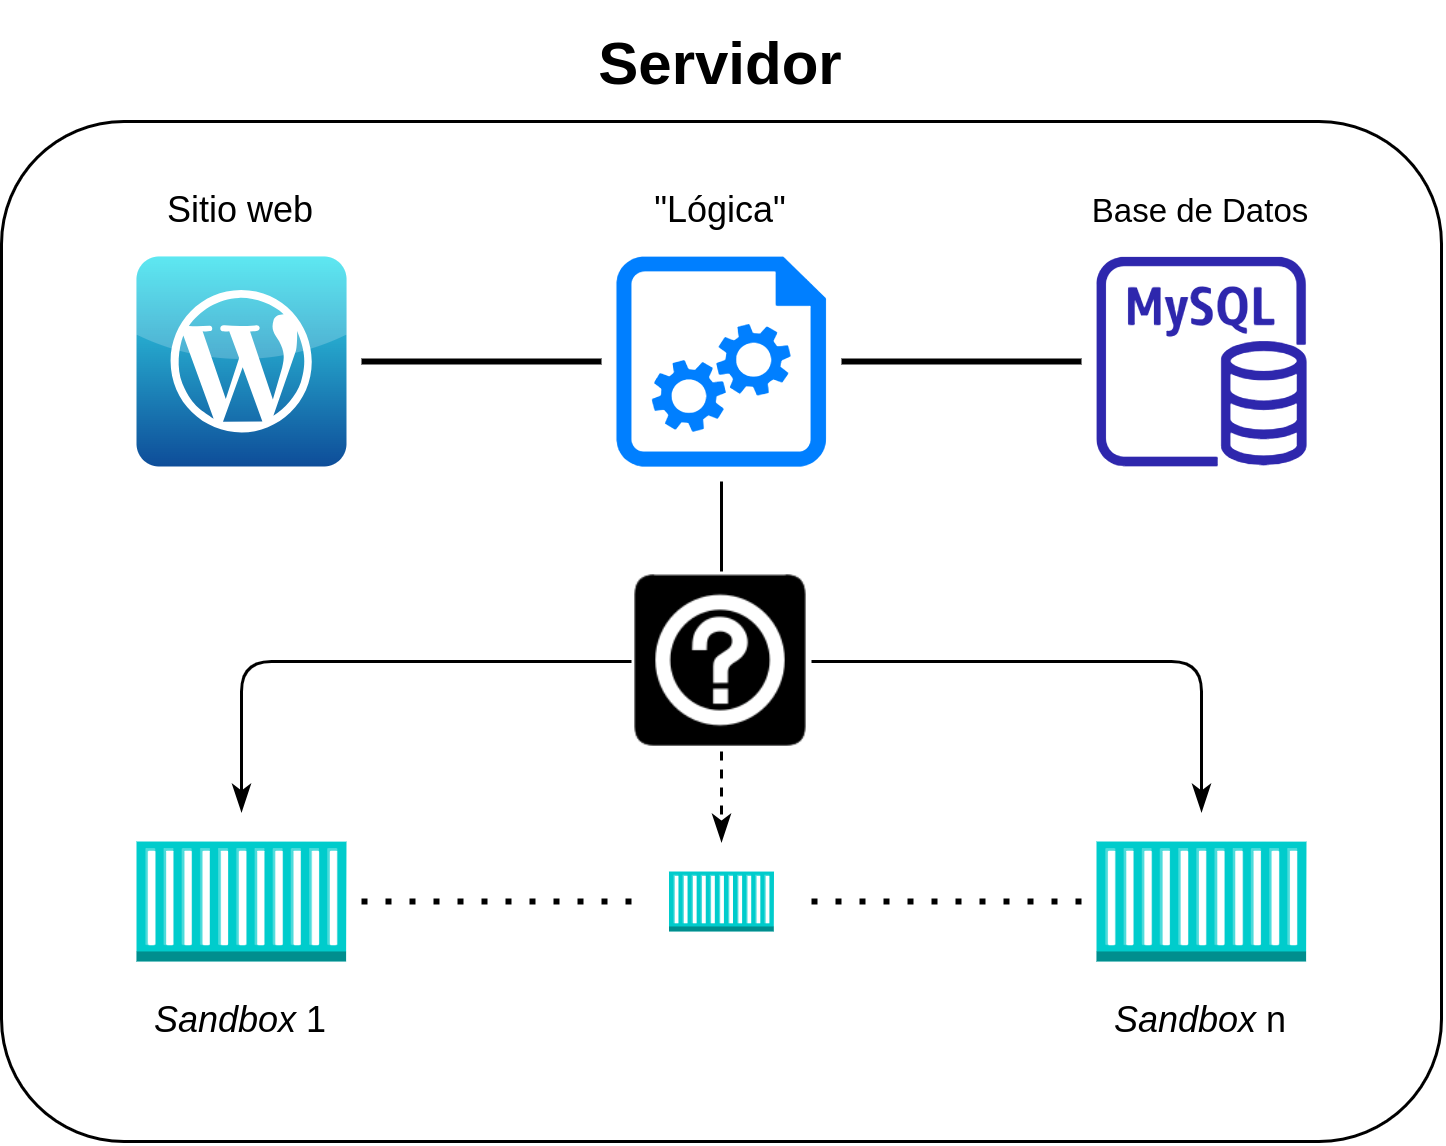
\includegraphics[scale=0.1]{images/diagramas/conexion.png}
            
            \column{.5\textwidth}
                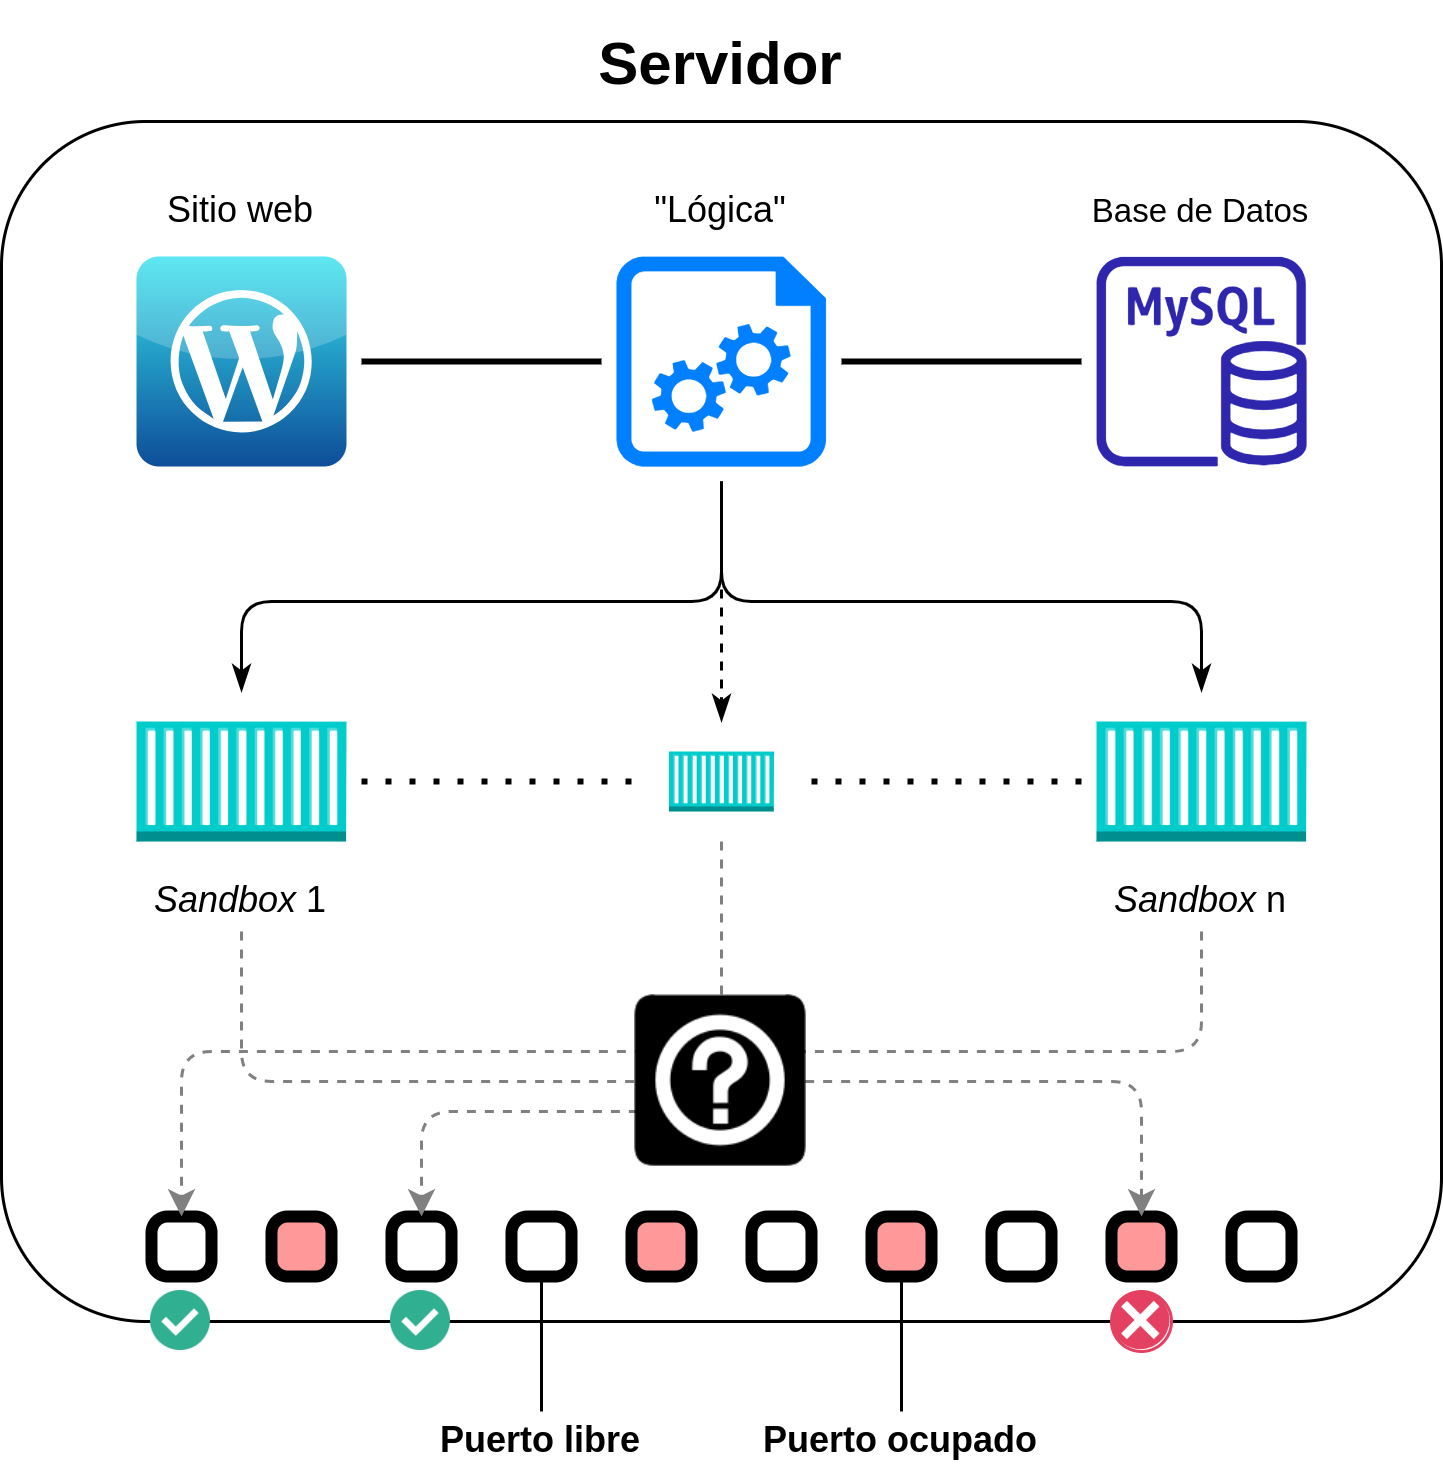
\includegraphics[scale=0.1]{images/diagramas/puertos.png}
        \end{columns}

        \begin{columns}[c]
            \column{.5\textwidth}
                \\
                \texttt{exec("docker run (...)")}
            
            \column{.5\textwidth}
                \\
                Gestión de puertos usando PHP
        \end{columns}
    \end{frame}

    \begin{frame}{Limitaciones del uso de contenedores Docker}
        \begin{itemize}
            \item Herramientas con interfaces gráficas (GUI)
            \\~\\
            \item Definición de puertos en el arranque del contenedor
        \end{itemize}
    \end{frame}

    \begin{frame}{Procesos bajo el usuario \texttt{www-data}}
        \begin{itemize}
            \item Pertenencia al grupo \texttt{docker}
            \\~\\
            \item Ejecución del servicio de Docker
            \\~\\
            \item Ejecución de la tarea de cron
        \end{itemize}
    \end{frame}

    
\section{Código auxiliar}

    \begin{frame}
        \Huge{\centerline{Código auxiliar}}
    \end{frame}

    \begin{frame}{Scripts de despliegue}
        \begin{columns}[c]
            \column{.55\textwidth}
                \begin{block}{\texttt{instalar.sh}}
                    \begin{enumerate}
                        \item Obtiene los laboratorios
                        \item Revisa los contenedores Docker
                        \item Si ya existe, lo actualiza.
                        \item Si no existe, lo construye.
                    \end{enumerate}
                \end{block}
            
            \column{.45\textwidth}
                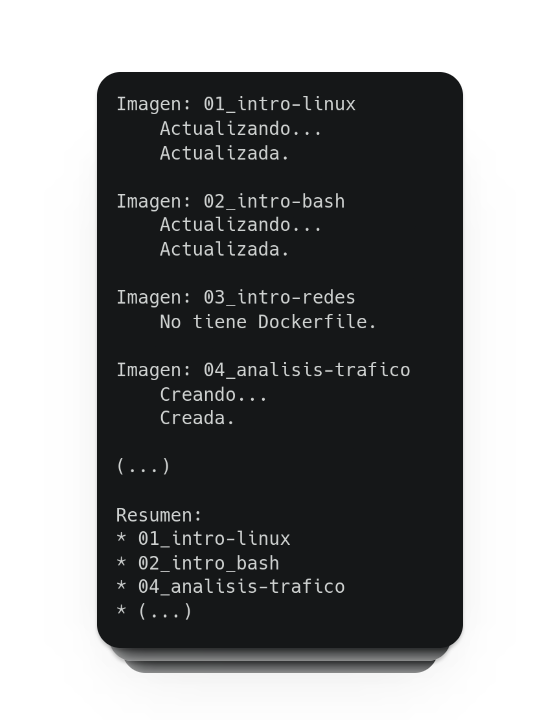
\includegraphics[scale=0.2]{images/capturas/instalar.png}
        \end{columns}
    \end{frame}

    \begin{frame}
        \begin{columns}[c]
            \column{.45\textwidth}
                \begin{block}{\texttt{stop-1h-container.sh}}
                    \scriptsize

            \begin{enumerate}
                \item {Obtiene los contenedores\\y su fecha de inicio}
                \item Para cada uno:
                \item Si pasó 1 hora, lo destruye.
                \item Muestra un mensaje informativo.
            \end{enumerate}
                \end{block}
            
            \column{.55\textwidth}
                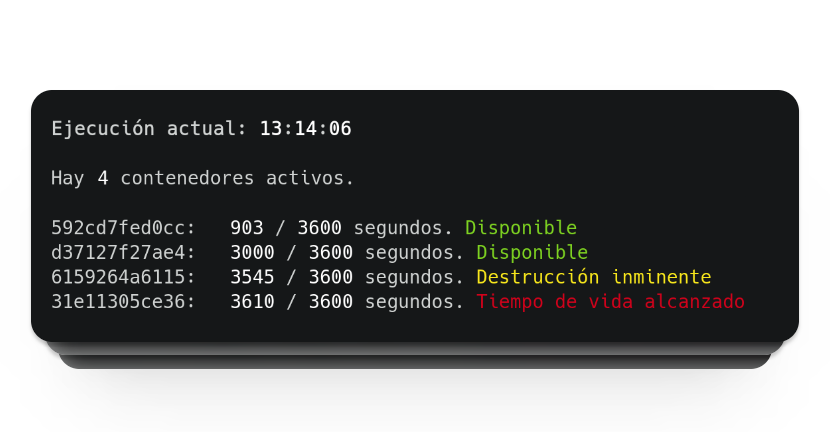
\includegraphics[scale=0.2]{images/capturas/cron.png}
        \end{columns}
    \end{frame}

    \begin{frame}{Proyectos para laboratorios}
        \begin{center}
            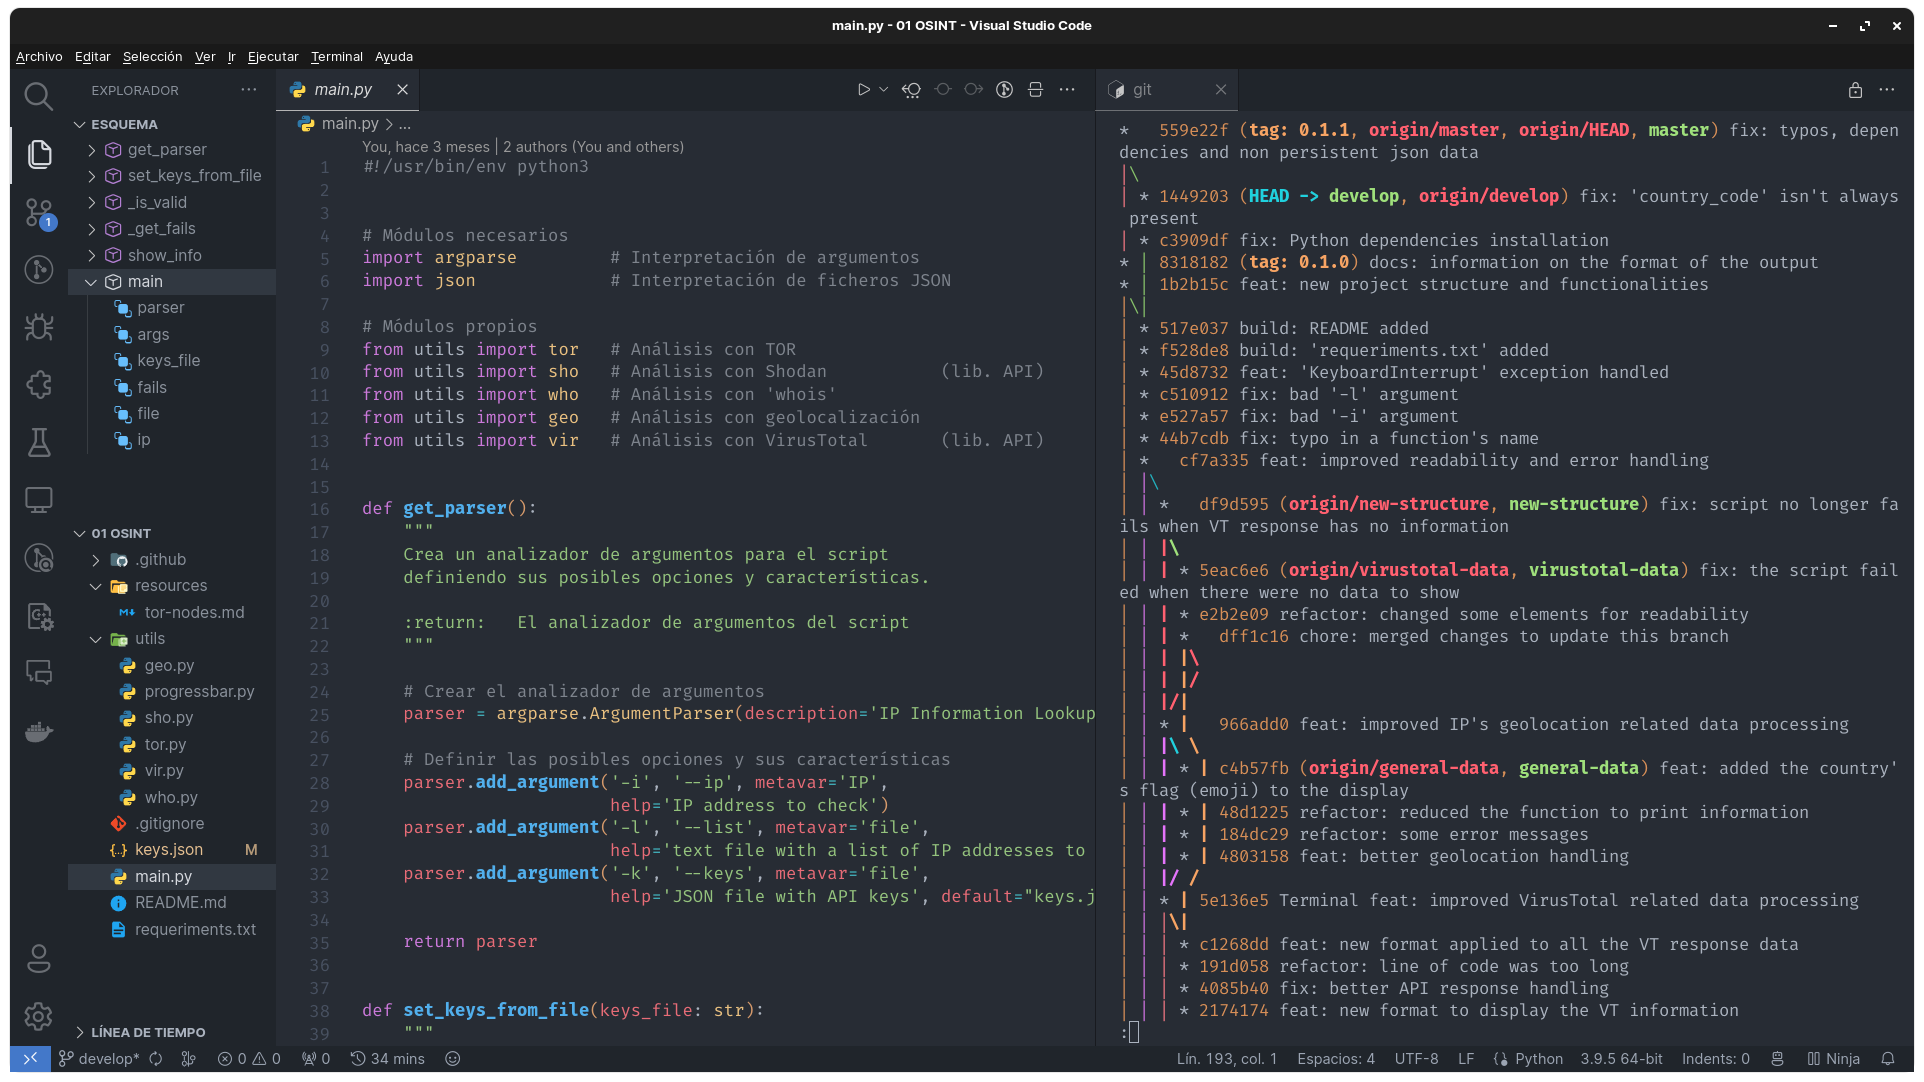
\includegraphics[scale=0.1]{images/capturas/vscode/ip-osint.png}
        \end{center}

        \begin{block}{\texttt{ip-osint/}}
            Proyecto escrito en Python que recibe una IP o lista de IPs y devuelve información sobre ellas obtenidas de diversas fuentes.
        \end{block}
    \end{frame}

    \begin{frame}
        \begin{center}
            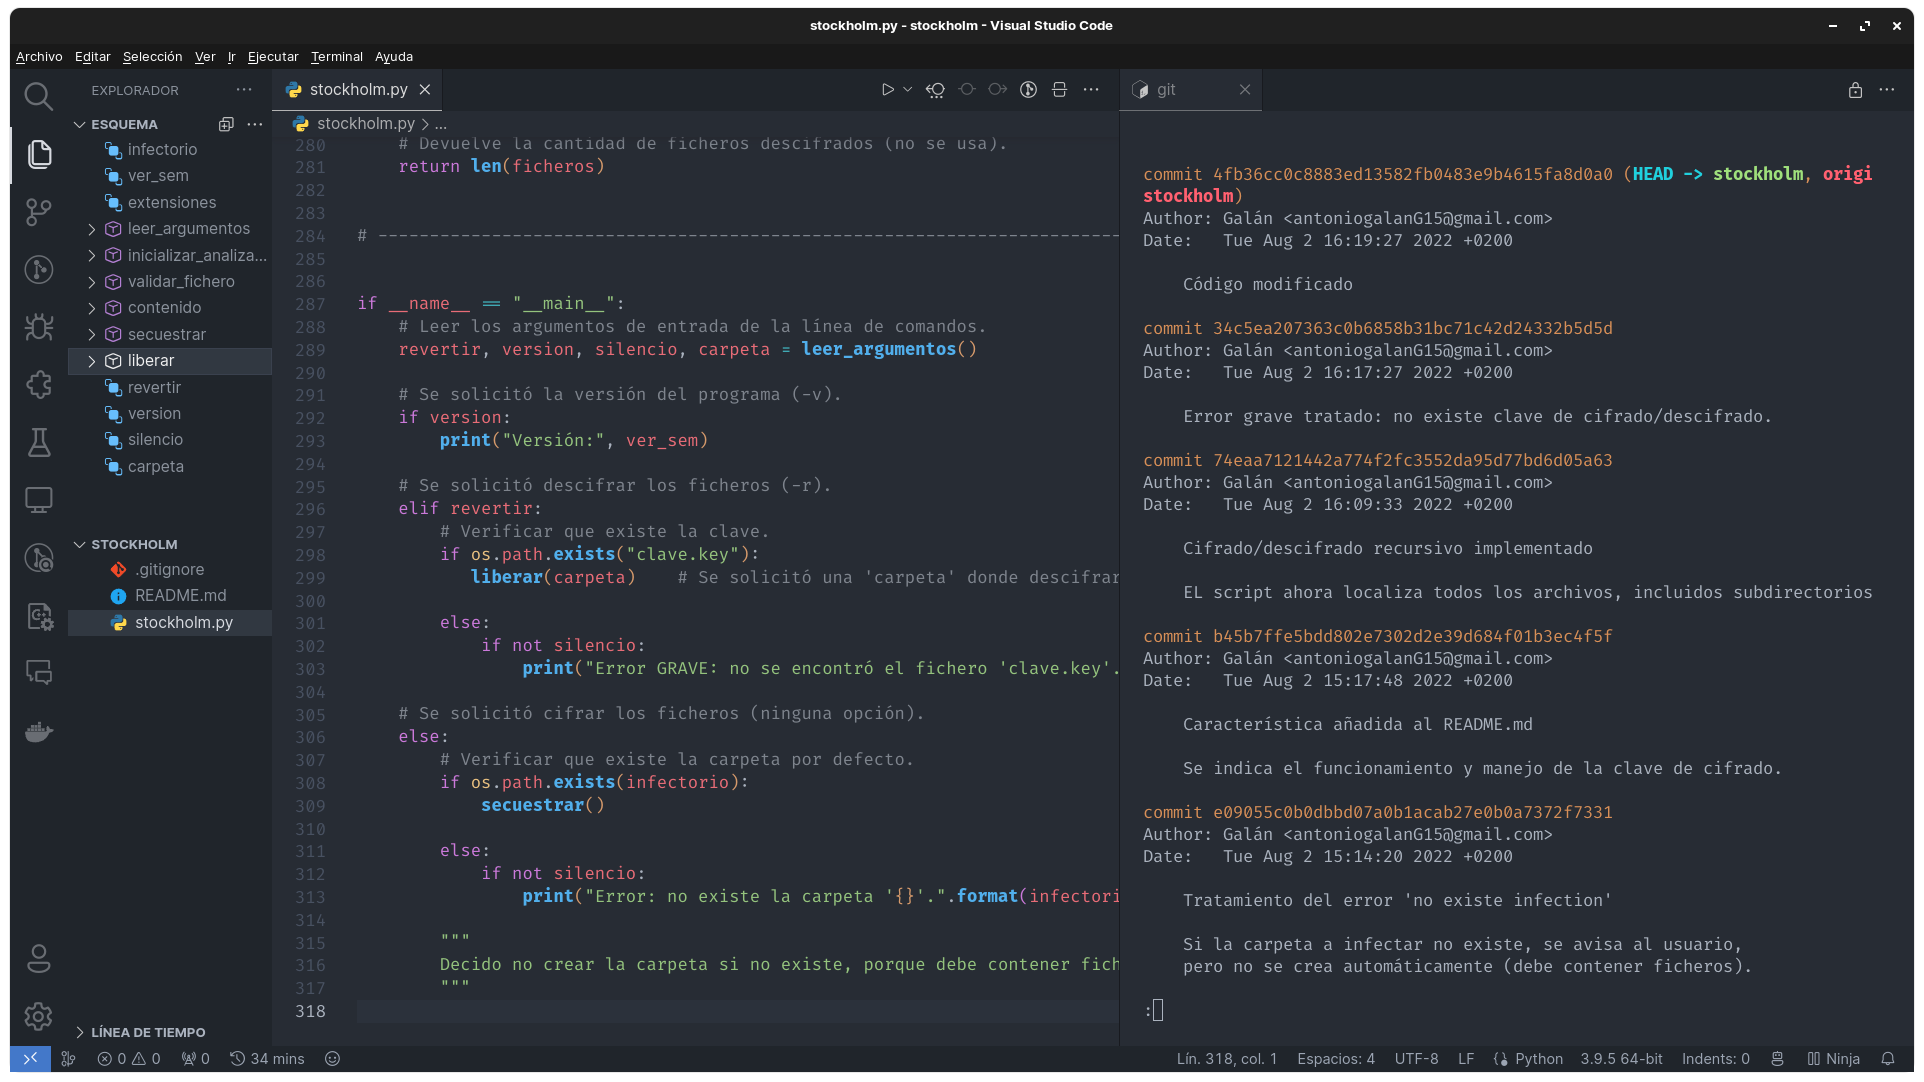
\includegraphics[scale=0.125]{images/capturas/vscode/stockholm.png}
        \end{center}

        \begin{block}{\texttt{stockholm.py}}
            Script escrito en Python que cifra (y descifra) los ficheros de un directorio específico del sistema, simulando un ransomware.
        \end{block}
    \end{frame}

    \begin{frame}
        \Huge{\centerline{Muchas gracias}}
    \end{frame}
